\chapter{Allgemeine}

\asypmtote\cite{Asymptote} ist eine Programmiersprache um Graphiken, vor allen aber nicht ausschließlich geometrische Konstruktionen zu erstellen.
Das Paket \optik{} wurde mit dem Ziel, die Erstellung von gängigen optische Diagramme in der Programmiersprache \asypmtote{} zu erleichtern, geschrieben.

Das Paket kann man aus der Git-Repository \url{https://github.com/hpb-htw/optik} herunterladen.
Es ist empfohlen, das Paket entweder via Git-Klone bei einem Non-Git-Projekt oder via Git-Submodule bei einem Git-Projekt einzubinden:

\begin{shellcode}
#  cd to your Project directory
## For a none-git-project: Just clone the last revision
git clone --depth 1 https://github.com/hpb-htw/optik.git
## For a git project
git submodule add --depth 1 https://github.com/hpb-htw/optik.git
\end{shellcode}

Beispielen in diesem Dokument sind in \repo{} zu finden. 
Ein Beispiel fängt --wenn nicht anders erwähnt-- mit folgenden Zeilen an:

\begin{asycode}
settings.tex="lualatex";  // input Unicode character directly from keyboard
settings.outformat="pdf"; // use PDF as default output

texpreamble("\newcommand{\pLabel}[1]{\mathsf{#1}}
\newcommand{\tLabel}[1]{\textsf{#1}}
"); // optional

unitsize(2mm);                       // justify size / scale of image

import geometry;                     // Optik uses this package.
import "optik/optik.asy" as optik;   // the path to the file `optik.asy' must be adjusted.
\end{asycode}


Der Inhalt der Datei \verb|shortcut.tex| ist wie folgt:

\begin{texcode}
\newcommand{\pLabel}[1]{\mathsf{#1}}
\newcommand{\tLabel}[1]{\textsf{#1}}
\end{texcode}


Die obigen Code-Auszüge lassen darauf schließen, 
dass eine funktionierende Installation von \LaTeX{} und \asypmtote{} die notwendige Voraussetzung für die Nutzung des Paket \optik{} ist.



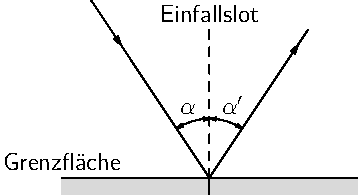
\includegraphics{asy/mirror-simple}
%
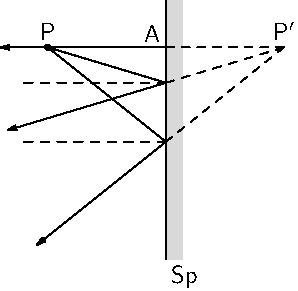
\includegraphics{asy/mirror-vertical}


